\documentclass[12pt]{article}
\usepackage{amsfonts,amsmath,amssymb, listings}

\usepackage[utf8]{inputenc}
\usepackage{graphicx}
\usepackage{multirow}
\usepackage{xcolor}

\usepackage{threeparttable}
\usepackage{blindtext}


\usepackage[a4paper, total={6in, 8in}]{geometry}

\usepackage[numbered,framed]{matlab-prettifier}
%\usepackage{color}

%\setcounter{MaxMatrixCols}{10}

\def\stackunder#1#2{\mathrel{\mathop{#2}\limits_{#1}}}%

\newcommand{\fiid}{\func{i.i.d.}} % use this as in: X_i \stackrel{\fiid}{\sim} \func{Exp} \left( \lambda \right)
\DeclareMathOperator{\Norm}{N}

\newcommand{\platzo}{\vspace*{2cm}}
\newcommand{\platzt}{\vspace*{4cm}}

\newcommand{\findep}{\func{ind}}  % could use indep instead if ind, but 1st book uses ind.

\newcommand{\R}{\ensuremath{{\mathbb R}}}
\newcommand{\N}{\ensuremath{{\mathbb N}}}
\def\QATOP#1#2{{#1 \atop #2}}
\def\QTATOP#1#2{{\textstyle {#1 \atop #2}}}
\def\QDATOP#1#2{{\displaystyle {#1 \atop #2}}}
\voffset=-2.54cm\hoffset=-2.54cm \textheight27cm \textwidth17.0cm \topmargin0.5cm
\oddsidemargin2.00cm \evensidemargin2.00cm \unitlength1cm

\def\func#1{\mathop{\rm #1}}%
\def\dint{\mathop{\displaystyle \int}}%
\newcommand{\Ind}{\ensuremath{{\mathbb I}}} % indicator function
\newcommand{\E}{\ensuremath{{\mathbb E}}} % expected value
\newcommand{\Var}{\ensuremath{{\mathbb V}}} % variance

\setlength{\parindent}{0pt}

\usepackage{float}

\newfloat{Program}{thp}{lop}[section]
\floatname{Program}{Program Listing}

\begin{document}

\pagestyle{empty}

\bigskip

\begin{figure}[htp]
    \centering
    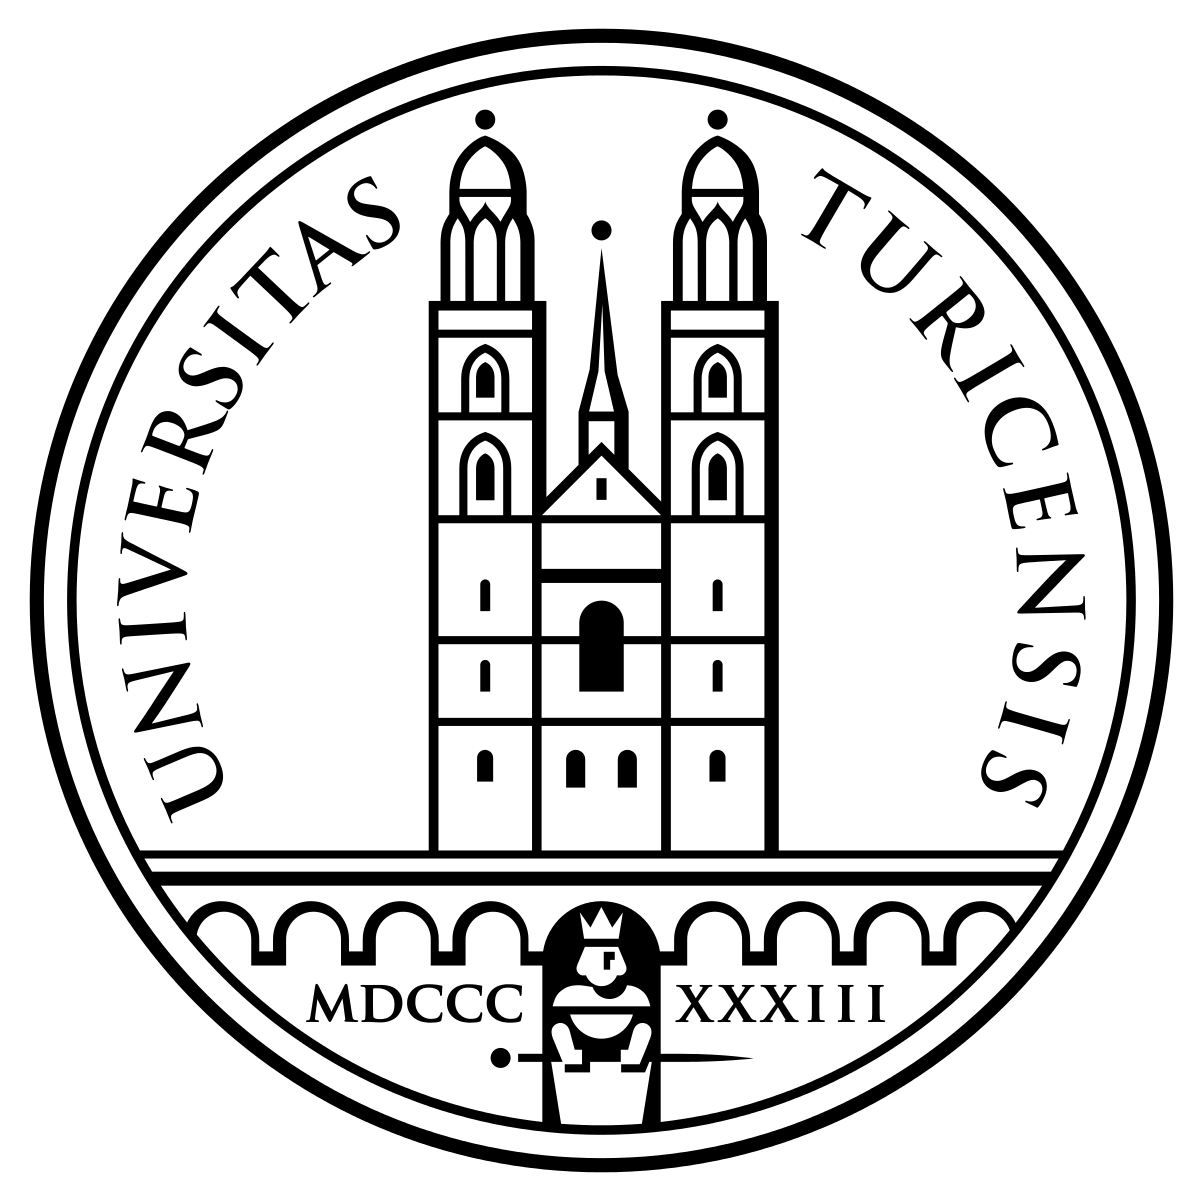
\includegraphics[width=4cm]{uzh logo 2.png}
    \label{fig:UZH}
\end{figure}

\begin{Large}
	\begin{center}
		\textbf{Digital Tools for Finance}
	\end{center}
\end{Large}

\vspace{2cm}

\begin{large}	
	\begin{center}
		\textbf{Effect of Interest Rate Changes on Cryptocurrencies} \vspace{0.1cm} \\ {Prof. Igor Pozdeev } \vspace{2cm} \\ \textbf{Matthias Olieslagers - 22714034}  \\ \textbf{
Cameron Storey - 22740815} \\
        \textbf{Marc David Parker - 22727762}\\
        \textbf{Qian Chen - 21742226}\\
	\end{center}
\end{large}

\tableofcontents

\newpage

\bigskip
\section{Introduction}

The goal of this research report is to discover how changes in FED interest rates have an impact on the prices of cryptocurrencies (e.g. Bitcoin) \newline
The up-front hypothesis, based on our knowledge of the financial markets is that the higher the FED interest rate goes, the lower the crypto prices will drop, i.e. they have a negative correlation. In this report, an attempt will be made to  confirm (or invalidate) the hypothesis statement above. \newline
In the first section, the different data sources will be covered. What does the data exactly represent and why is it relevant to look into for this particular research. In the second part, the methodology will be laid out. Lastly, the results will be critically evaluated and interpreted and a final conclusion will be provided. 

\section{Data}

The datasets that were used to develop an answer to this research question are the BTC-USD Daily Price and the FED rate, both over the extensive time period from 2016 to date. At first, we also looked at several other currencies such as Solana and the Dogecoin, but decided not to include them in the final analysis as their values are less representative for the market. We also looked at other interest rate metrics, such as the LIBOR and SOFR rate. These two interest rates relatively close follow the path of the FED rate and they are both continuous rates. All of the data was obtained from reliable sources such as Yahoo Finance and MarketWatch.

\begin{Program}[!htb]
\begin{lstlisting}[style=Matlab-editor,basicstyle=\mlttfamily\footnotesize]
dummy
  
\end{lstlisting}
\caption{Dummy code}
\label{Dummy code}
\end{Program}

\section{Explanation about the first notebook 'Analysis'}
\subsection{Methodology}
In this paragraph, we will dig deeper on the methodology for the analysis and explain and interpret the results. The extensive explanation (e.g. all of the underlying code, plots etc.) can be found in the Jupyter notebook, this report serves as a brief summary of the main findings. \newline \newline
The programming language Python, with extensions pandas, numpy and matplotlib, is used and the following approach is used. First, we read in the BTC and FED data and some of the functions for the calculation of metrics such as the Moving Average and Rolling Volatily are defined. These metrics will be used in the analysis later on. Next, the particular dates at which there was effectively a change in the FED rate are highlighted and sorted out, we will obviously focus on these particular dates when assessing what the effect of an interest change on the crypto prices is. \newline
\newline As an illustration, the graph below (see Figure \ref{fig:FED Rate evolution 2016 - 2022}) illustrates the evolution of the FED rate across the last 6 years. As can be seen, this is a stepwise function, so there are no daily changes but rather periodical changes with flat periods in between. \newline It is interesting to note that the macro-economic events can clearly be seen in the graph. At the beginning of 2020, the interest rate drops to a low point in order to support the economy during the Covid-19 outbreak. Now since the beginning of 2022, the interest rate has started to rise sharply in order to slow down the inflation. The FED rate is thus a tool to regulate the economy and in the next paragraph down below we will discuss whether these changes have any significant impact on the prices of BTC.

\begin{figure}[!htb]
   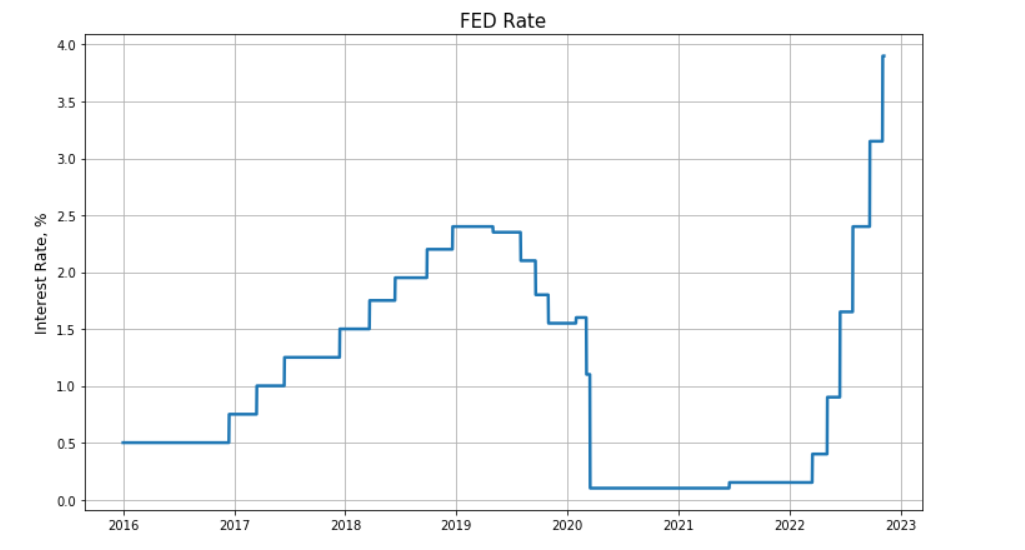
\includegraphics[scale=0.7]{research_project/text/paper/FED rate graph.png}
   \centering
   \caption{FED Rate evolution 2016 - 2022}
   \label{fig:FED Rate evolution 2016 - 2022}
\end{figure}


\subsection{Results}
First we looked at the FED rate changes and if there is an n-day correlation after these changes had taken place for n=1,2,...,7.
\begin{figure}[H]
   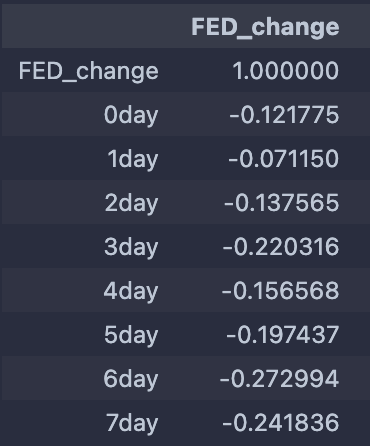
\includegraphics[scale=0.7]{research_project/text/paper/1.png}
   \centering
   \caption{FED Rate changes and n day correlation}
   \label{fig:FED Rate evolution 2016 - 2022}
\end{figure}
From this we see that there is no significant relationship between a certain day after the change takes place and a movement in BTC price movements.\\

Because of this lack of significant results we will now examine if we see any results from the moving average. We plotted the moving averages against price as follows.
\begin{figure}[H]
   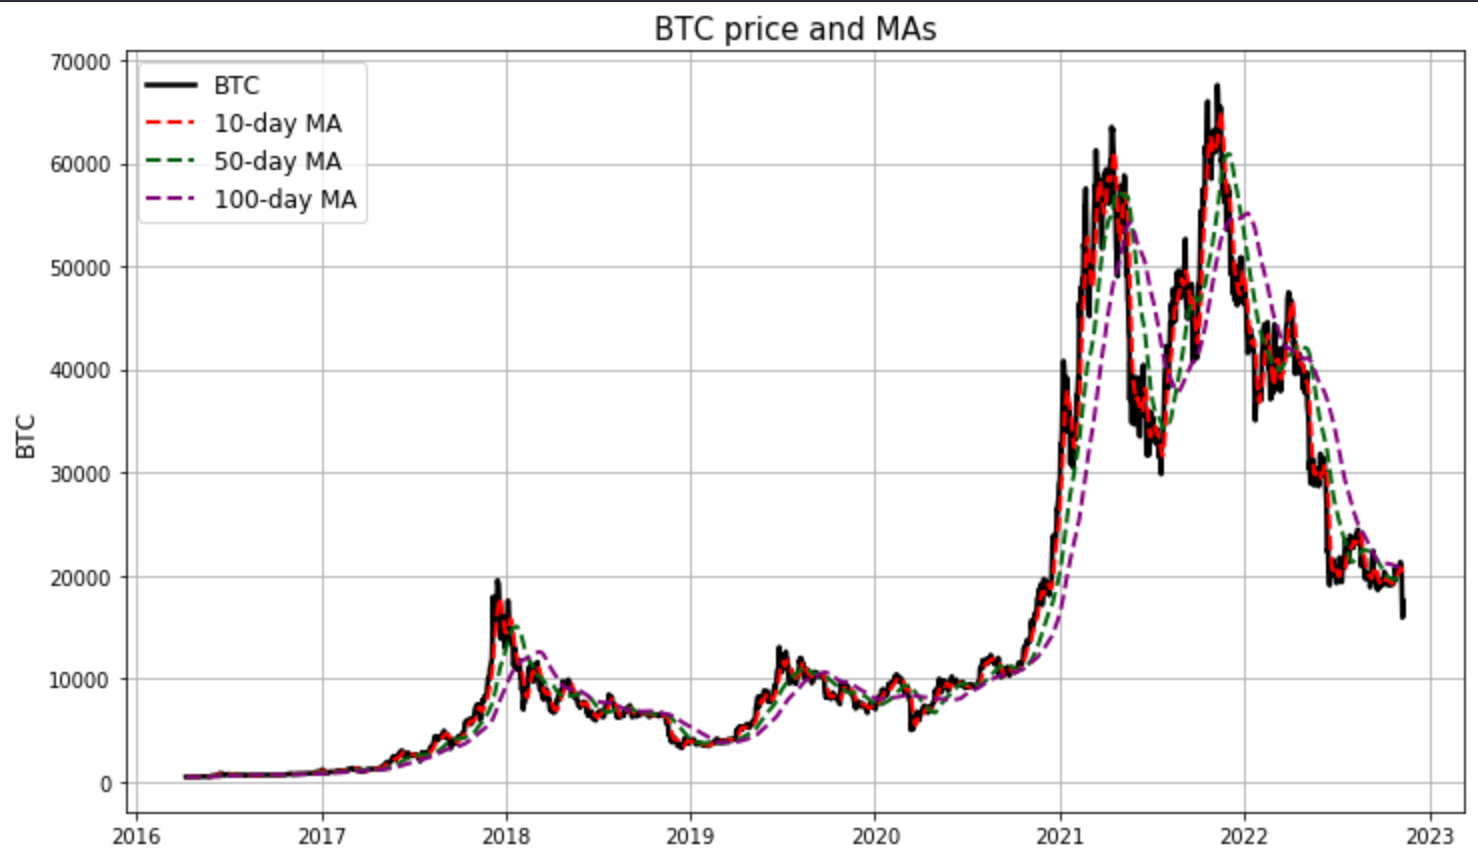
\includegraphics[scale=0.7]{research_project/text/paper/2.png}
   \centering
   \caption{Moving averages against price}
   \label{fig:FED Rate evolution 2016 - 2022}
\end{figure}
We checked whether the change in moving average after an announcement was "out of the ordinary", once again we had no significant findings. Due to the change in the nature of cryptocurrencies it was hard to use the same distribution on BTC from 2022 against that from 5 years ago.
\subsection{Volatility Analysis}
Because we observed no significant finding from the analysis in the previous section we have decided to analyse if the changes in FED rate make any difference on the volatility of BTC price.\\
Below is a graph showing BTC volatility.
\begin{figure}[H]
   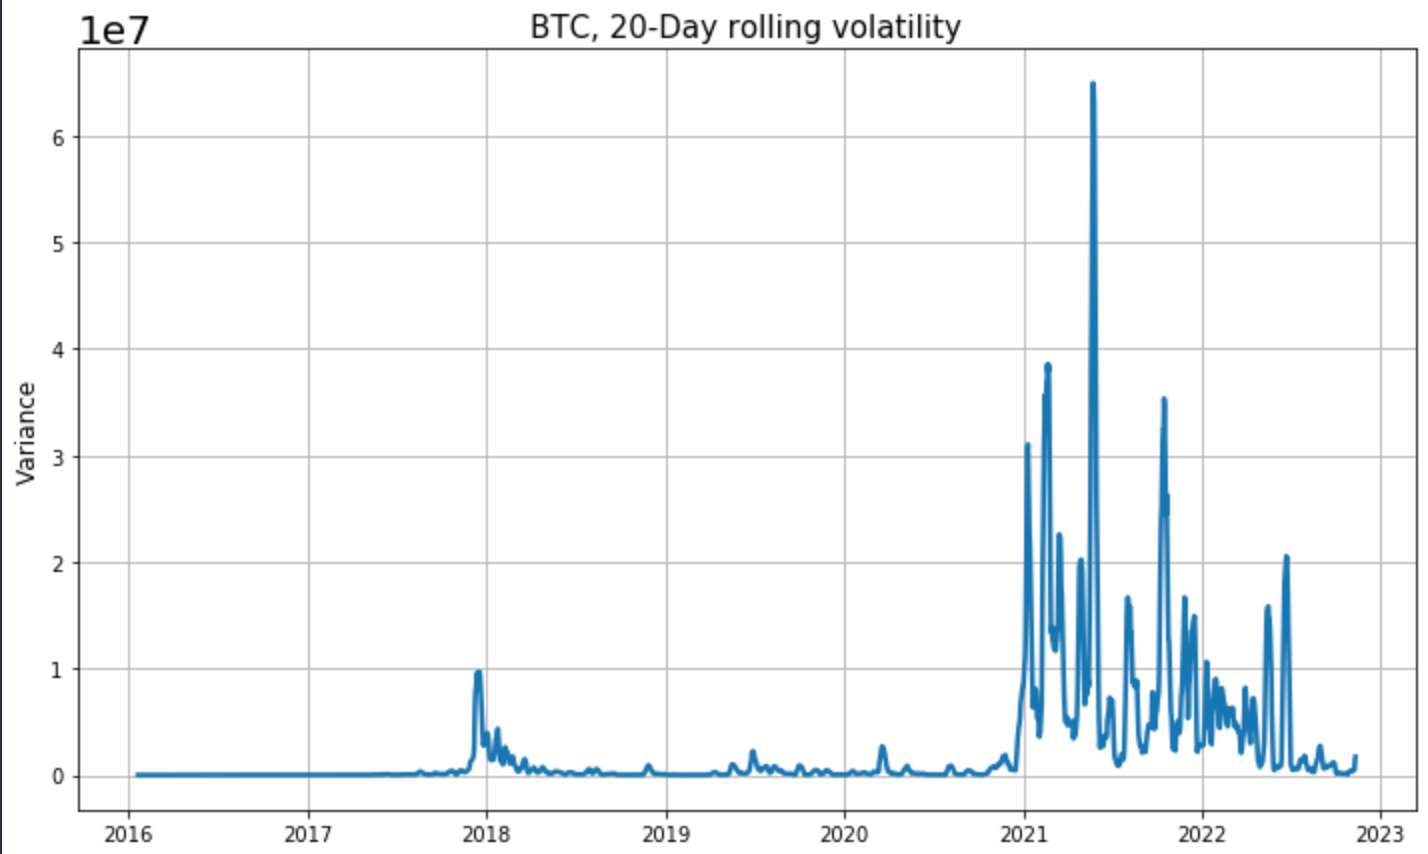
\includegraphics[scale=0.7]{research_project/text/paper/6.png}
   \centering
   \caption{BTC volatility}
   \label{fig:FED Rate evolution 2016 - 2022}
\end{figure}

\noindent We performed quantitative analysis on this and obtained the data as follows.

\begin{figure}[H]
   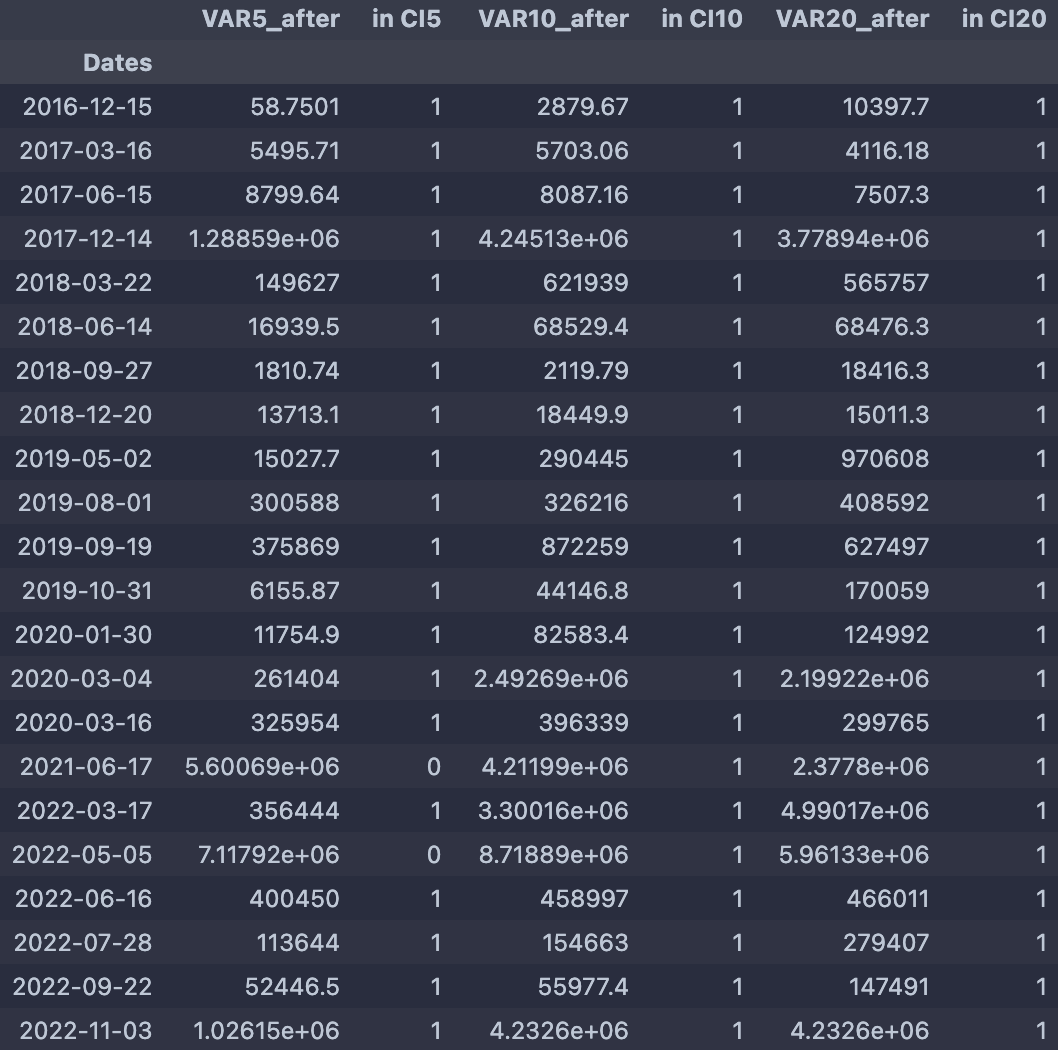
\includegraphics[scale=0.7]{research_project/text/paper/7.png}
   \centering
   \caption{BTC price Volatility}
   \label{fig:FED Rate evolution 2016 - 2022}
\end{figure}
Once again we see there is no significant evidence that a change in FED rate has any effect on the volatility of BTC prices.
\subsection{Daily Change}
Another metric we have decided to look at was the daily change, the daily high minus the daily low of the day. We will analyse the daily change in the days following a FED rate change.\\

The obtained data has been inserted below.
\begin{figure}[H]
   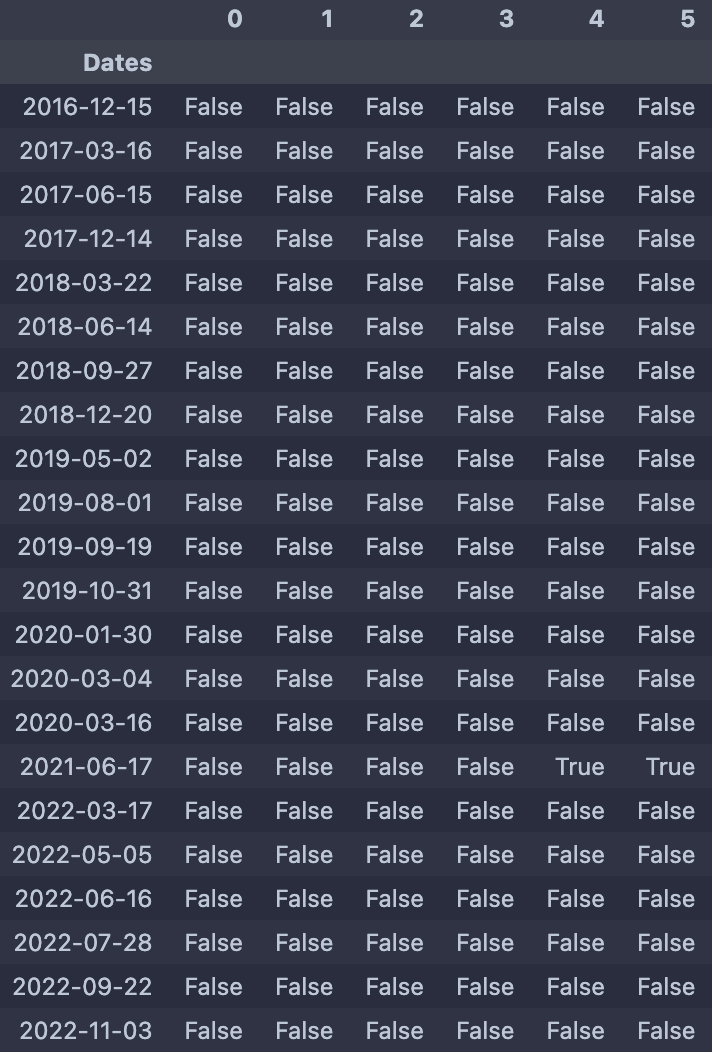
\includegraphics[scale=0.7]{research_project/text/paper/10.png}
   \centering
   \caption{Daily Change Significance}
   \label{fig:FED Rate evolution 2016 - 2022}
\end{figure}
Unlike before we have observed some significant values. We chose to ignore these as they are very close together and it is highly likely this significance has been caused by other factors in the cryptocurrency markets instead of the FED rate changing. We also struggle to make a comparison here as the daily changes in recent times are very different to that observed years ago due to the change in BTC price, we see much larger interdaily change now. 

\newpage
\section{LIBOR Analysis}
We also analysed the continous interest rate data using the LIBOR rate to observe if we saw any correlations.\\

After doing this we saw a strong negative correlation in BTC price and LIBOR in the short term, we observed a correlation coefficient of -0.896524, a strong negative correlation, we only analysed this over the past year in which we saw interest rates increasing and BTC price decreasing, we don't believe this is due to causation and is merely just a correlation due to external factors.
\section{Conclusion}
In conclusion from all the analysis we have conducted we have no reason to believe the FED rate changes have any real effect of the BTC price movement in the short or long term, from all the analysis we see no significant evidence that there is any correlation in price movements and the change in the FED rate. This leads to the conclusion that there are larger macro forces that influence the BTC price movements and we would be unable to make an informed decision on the future price movements of BTC based on the announcement of a FED rate change alone.

\end{document}
